\chapter{Design Rationale}

In this chapter we list and explain the reasoning for the design choices we have made for the lip-tracking library.

\section{Technologies}

A description of the technologies we used can be found in \Cref{technologies}. We chose these technologies because they are very common and well supported, in addition to being available on every platform with which we are working (Windows, Linux, OS X, Android). 

\section{Application Programming Interface}

We wanted to make our API as simple as possible for the user, while still being flexible. As a result, we allow images to be inputted in many common and popular formats. The full list of compatible image formats is as follows:

\begin{description}
  \item[Bitmaps] \texttt{*.bmp, *.dib}
  \item[JPEG files] \texttt{*.jpeg, *.jpg, *.jpe}
  \item[JPEG 2000 files] \texttt{*.jp2}
  \item[Portable Network Graphics] \texttt{*.png}
  \item[Portable image format] \texttt{*.pbm, *.pgm, *.ppm}
  \item[Sun rasters] \texttt{*.sr, *.ras}
  \item[TIFF files] \texttt{*.tiff, *.tif}
\end{description}

The user can also change the acceptance threshold for lip detection. If there are too many false positives, then the threshold can be lowered to compensate, and vice versa.

\section{Algorithm}

There are many different algorithms that have been used in the past for feature tracking. 
These can be divided into three categories, geometric-based approaches, appearance-based approaches, and model-based approaches. Ahmad Hassanat has provided a literature review comparing these approaches in his paper \textit{Visual Speech Recognition}~\cite{Hassanat14}.

\subsection{Geometric-Based Approaches}

These approaches involve edge detection and then trying to match ratios of the edge's height, width, area and perimeter with some predefined values.

\subsection{Appearance-Based Approaches}

These approaches involve color segmentation of the image and then trying to match a segment with a predefined set of colors. 
This is the most common approach currently taken~\cite{Stillittano13}\cite{Yang09}, but does not always have good results. Increasing the contrast beforehand can somewhat improve the results.

\subsection{Model-Based Approaches}

These approaches involve creating a statistical model of a feature shape by inputting a set of hand-landmarked images into a neural network.
This model can then be used to very accurately find a similar shape in an image. 
There are three common model-based approaches, the Active Contour Model (ACM), Active Shape Model (ASM), and Active Appearance Model (AAM).
These three models are closely related in that they all use the same fundamental algorithm. However, ASM is an improvement over ACM and AAM is an improvement over ASM. These improvements bring more accuracy to the algorithm, however, they also increase complexity and runtime.

Additionally, both ASM~\cite{Li09} and AAM~\cite{Wang14} have been shown to be parallelizable with CUDA.
	

\subsection{Our Approach}

We have chosen to take a hybrid approach that combines all three previous approaches. The geometric-based and appearance-based approaches alone do not produce results that are accurate enough for us. They run very quickly, however, and can produce a better input image for a model-based approach. The model-based approach we are using is the Active Shape Model. The model is a good balance between the Active Contour Model, which is too simple and not accurate enough, and the Active Appearance Model, which is complicated and relatively slow. We will also convert all of the input images to grayscale as this will speed up many of the processing operations. An example of all the operations we will perform can be found in \Cref{fig:lena}.

\begin{figure}[p]
    \centering
    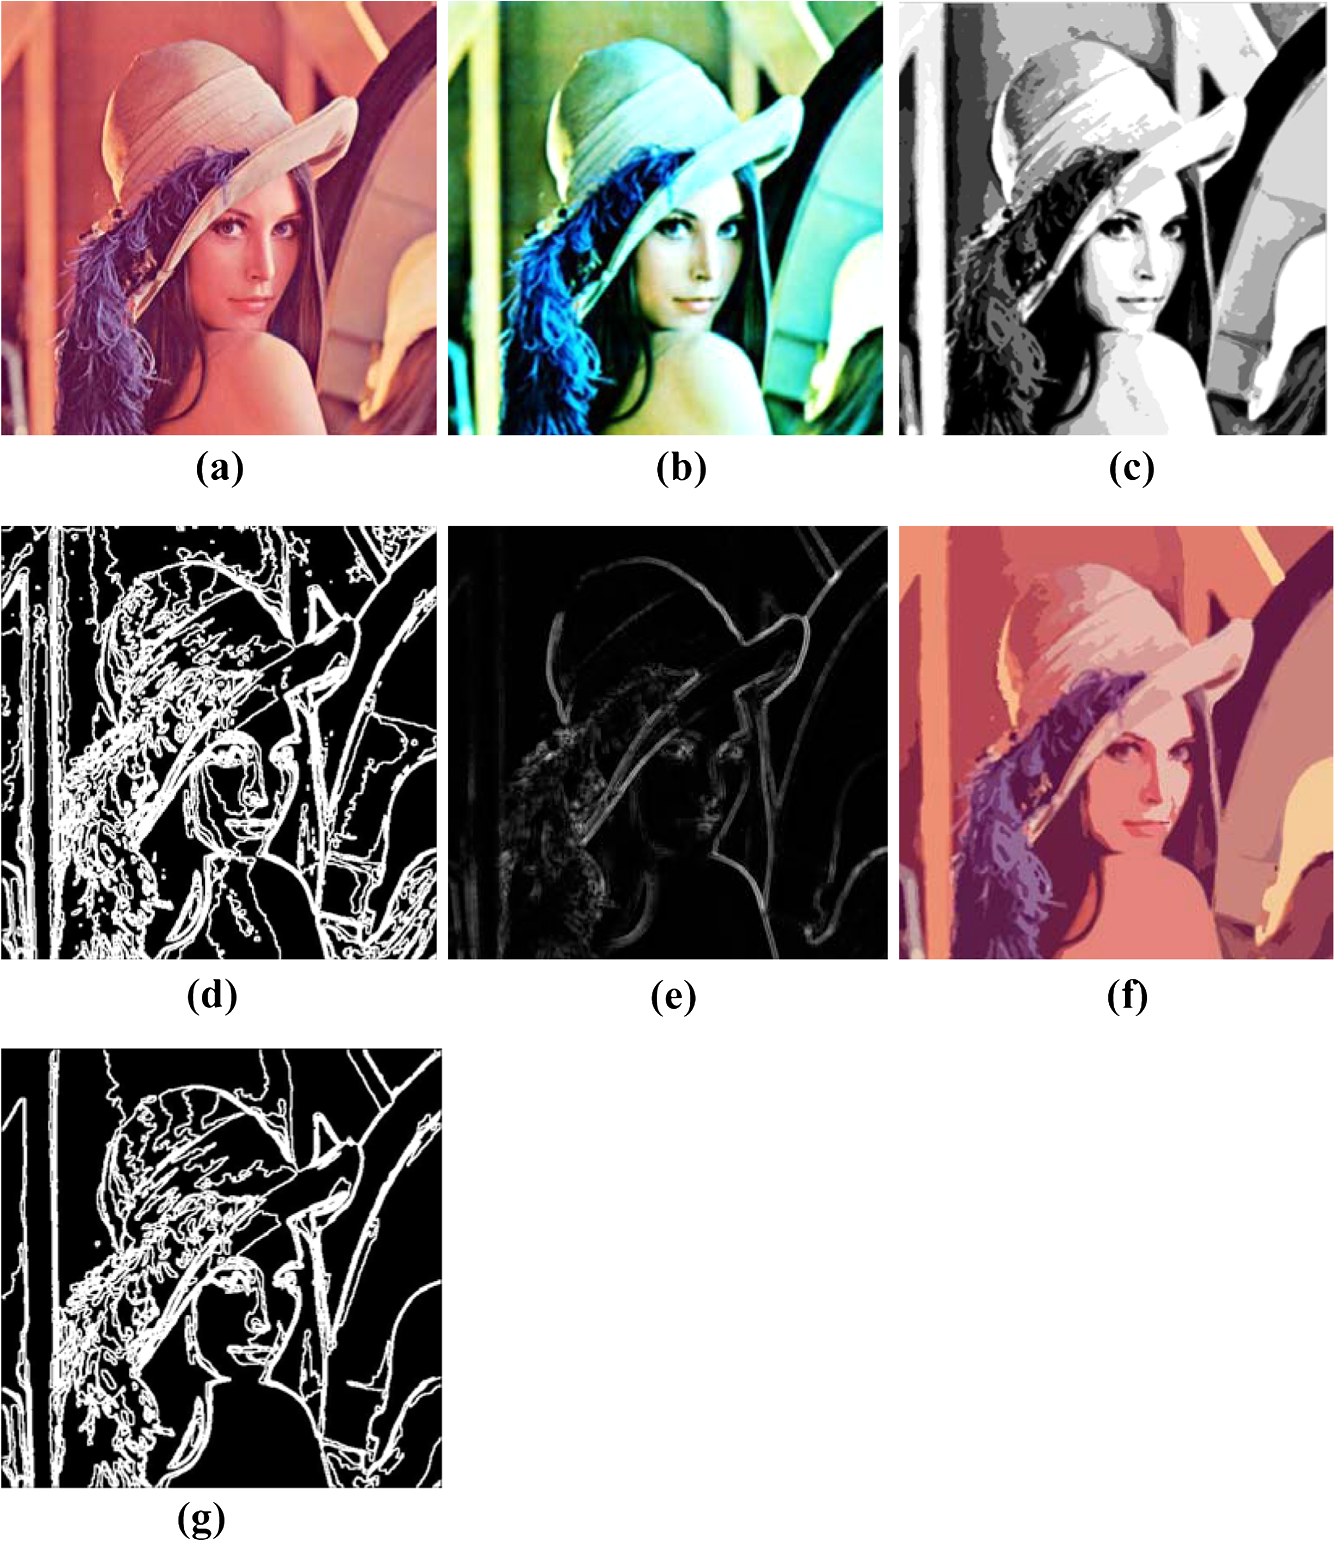
\includegraphics[width=0.8\textwidth]{diagrams/lena.png}
    \caption[Image filters]{(a) Source image\\(b) Increased contrast\\(c) Grayscale\\(d) Heavy edge detection\\
	(e) Light edge detection\\(f) Color segmentation\\(g) Medium edge detection\\Figure taken from Zhang\cite{filters}}
    \label{fig:lena}
\end{figure}